\chapter{Neural Networks}
\label{chapter:nn}

Neural networks use one particular architecture for computing.  This
architecture is inspired by animal brains where billions of neurons are connected.
This assignment does not intend to explain what neural networks are,
how they resemble brains, and biological experiments discovering the
mechanisms of brain functions.  Instead, this explanation focuses on
using the architecture solving relatively simple problems: creating
logic gates.

\begin{figure}[h]
\centering
{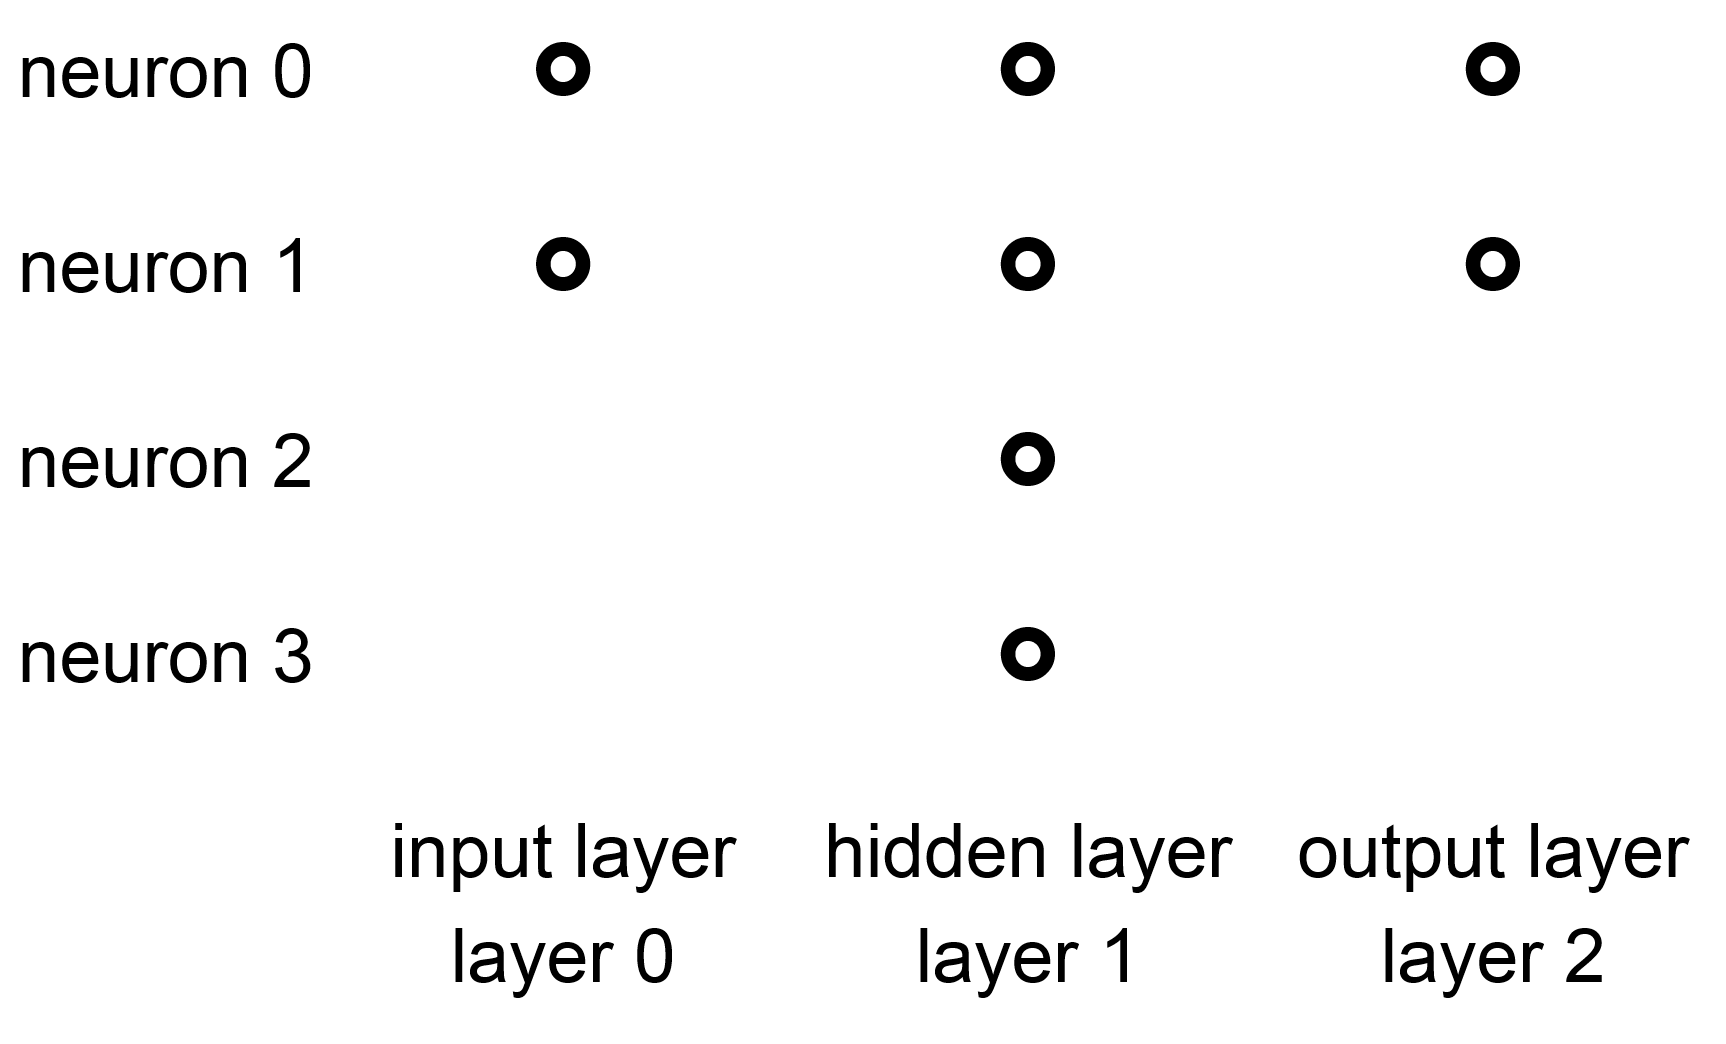
\includegraphics[width=4in]{\thischapterpath/figures/layers.png}}
\caption{Layers of a neural network.}
  \label{fig:layers}
\end{figure}

This assignment uses a neural network with three layers: one input
layer (layer 0), one hidden layer (layer 1), and one output layer
(layer 2).  Figure~\ref{fig:layers} shows the structure.  The input
layer has two neurons (neurons 0-1), the hidden layer has four neurons
(neurons 0-3), and the output layer has two neurons (neurons 0-1).

\begin{figure}[h]
\centering
\subfigure[]
{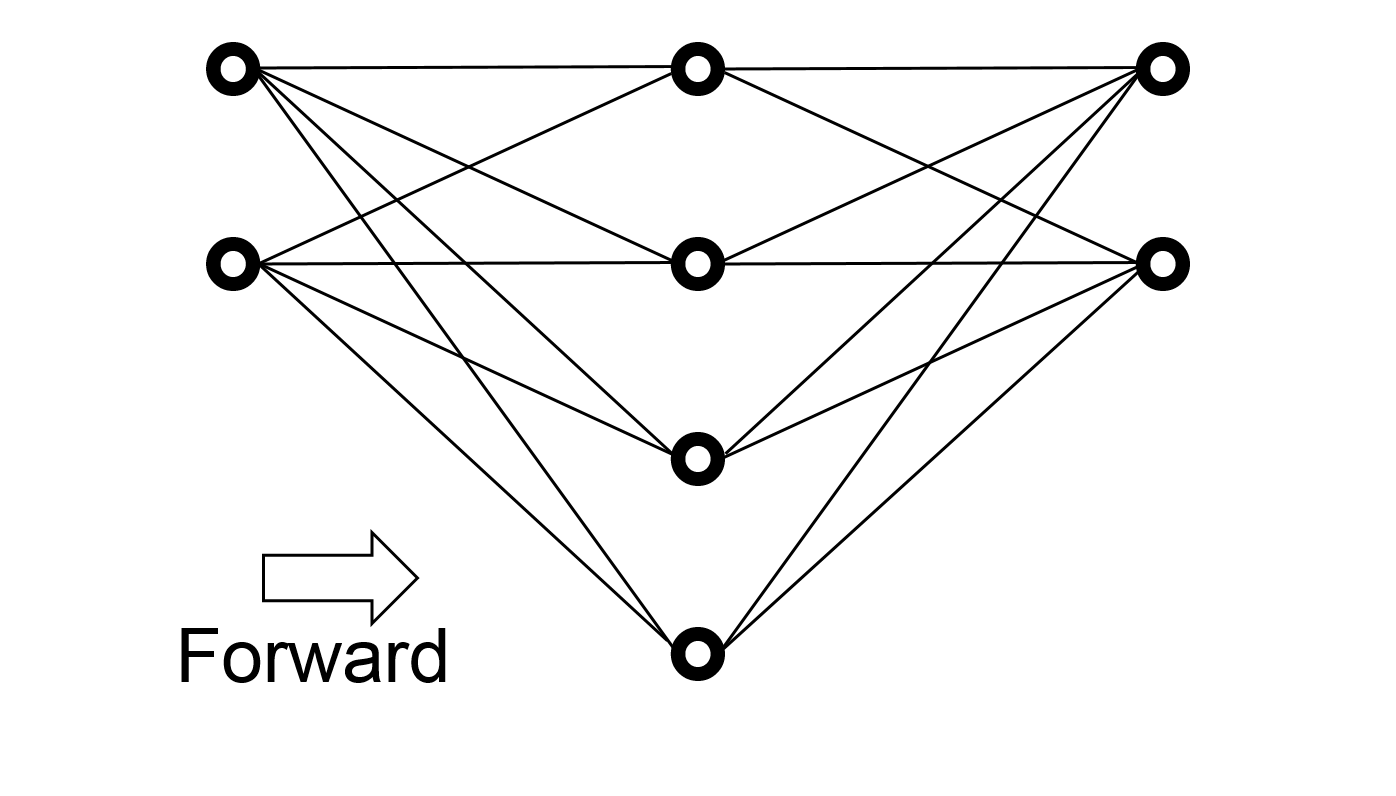
\includegraphics[width=3in]{\thischapterpath/figures/forward.png}}
\hspace{0.3in}
\subfigure[]
{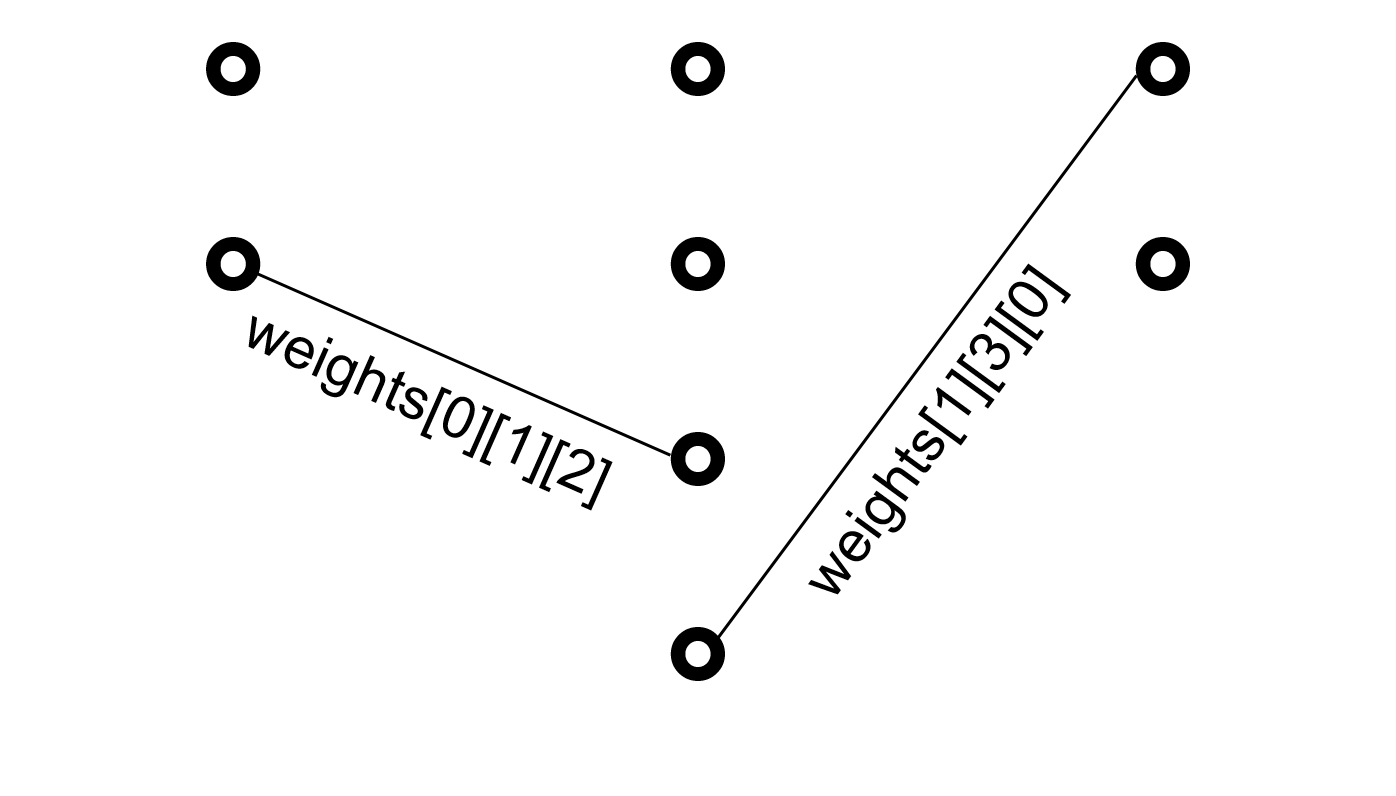
\includegraphics[width=3in]{\thischapterpath/figures/weights.png}}
\caption{(a) Information moves from left to right.
(b) The definition of the indexes.}
  \label{fig:forward}
\end{figure}

Information moves from the layers on the left toward the layers on the
right.  {\it There is no feedback of information.  Nor do two neurons
of the same layer exchange information.  } Figure~\ref{fig:forward}
(a) connects neurons of different layers.  These are the only
connections between enurons.

The neurons in two adjacent layers are connected by {\it weights}.  In
this assignment, weights are expressed as a three-dimensional array:

\begin{verbatim}
weights[l][s][d]
\end{verbatim}

connects the neuron {\tt s} (source) at layers {\tt l} to neuron {\tt
d} (destination) at {\tt l + 1}.  In the following sections, it is
written as $w_{l, s, d}$.

\section{Computation in Neural Networks}

The hidden and the output layers are further divided into two parts:
The first combines the numeric inputs from the previous layer. The
second takes the result from the first, converts the value using a
function, and makes the new value the input for the next layer.  More
specifically, the first part for neuron $d$ at layer $l$ is

\begin{equation}
\mathscr {\bf i}_{l, d} = 
b_{l, d} + \underset{s} {\Sigma}
(\mathscr {\bf o}_{l-1, s}
\cdot
w_{l-1, s, d}).
\end{equation}

The symbols are defined as follows:
\begin{itemize}[noitemsep,nolistsep]
\item $\mathscr {\bf i}_{l, d}$:  input of neuron $d$ at layer $l$.
\item $b_{l,d}$:  bias of neuron $d$ at layer $l$.
\item $\mathscr {\bf o}_{l-1, s}$: output of neuron {\tt s} at layer $l-1$.
When $l$ is zero, this is the input layer and $\mathscr {\bf o}_{l,
s}$ are the values given to the neural network.
\item $w_{l-1, s, d}$:  weight connecting neuron {\tt s} at layers $l-1$ to neuron {\tt
d} of $l$.
\item The range of $s$ is determined by the number of neurons at layer $l-1$.
\end{itemize}

Many functions have been proposed for converting $\mathscr {\bf i}_{l,
d}$ to $\mathscr {\bf o}_{l, d}$.  Among all options, the {\it
sigmoid} function,  expressed as $\sigma(x)$, is one of the most widely
used:

\begin{equation}
\sigma(x) = \frac{1}{1 + e^{-x}}.
\end{equation}

Thus,

\begin{equation}
\mathscr {\bf o}_{l, d}
= \sigma(\mathscr {\bf i}_{l,d})
\end{equation}

or

\begin{equation}
\mathscr {\bf o}_{l, d} = 
\frac{1}
{
  1 + e^
  {
    -(
        b_{l, d} + \underset{s} {\Sigma}
        (
           \mathscr {\bf o}_{l-1, s}
           \cdot
          w_{l-1, s, d}
        )
      )
  }
}.
\end{equation}

The $\sigma$ function has a special property: the derivative of
$\sigma(x)$ can be calculated easily:

\begin{equation}
\begin{array}{l}
\frac{d \sigma(x)}{d x} \\
=  \frac{d}{dx} (\frac{1}{1 + e^{-x}}) \\
= - \frac{1}{(1 + e^{-x})^2} \frac{d}{dx} (1 + e^{-x}) \\
=  \frac{e^{-x}}{(1 + e^{-x})^2} \\
= \frac{1}{1 + e^{-x}} \frac{e^{-x}}{1 + e^{-x}} \\
= \frac{1}{1 + e^{-x}} \frac{1 + e^{-x} - 1}{1 + e^{-x}} \\
= \sigma(x) (1 - \sigma(x)).
\end{array}
\label{eqn:derivativesigma}
\end{equation}

If the value of $\sigma(x)$ is $v$ for a particular
value of $x$, then the derivative of $\sigma(x)$ at this value of $x$
is $v (1-v)$.
With this definition, it is time to give an example shown in
Figure~\ref{fig:example1}.  
\begin{figure}[h]
\centering
{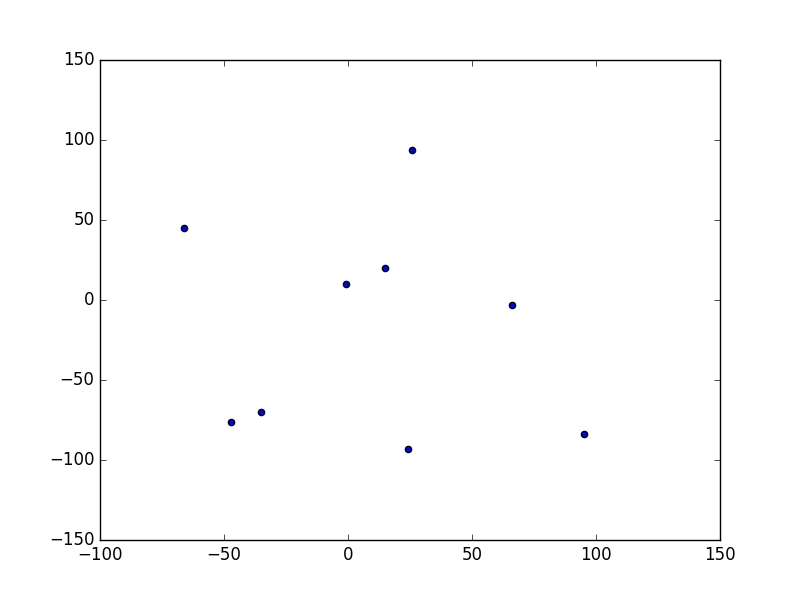
\includegraphics[width=3in]{\thischapterpath/figures/example1.png}}
\caption{Example caclulating a neuron's output.}
  \label{fig:example1}
\end{figure}

The input to neuron 1 at layer 1 is

\begin{equation}
0.3 + 0.99 \cdot 0.8 + 0.01 \cdot 0.2 = 1.094.
\end{equation}

After the sigmoid function, this neuron's output is

\begin{equation}
\frac{1}{1+ e^{-1.094}} = 0.7491342.
\end{equation}

Next, consider the  example in Figure~\ref{fig:example2}.

\begin{figure}[h]
\centering
{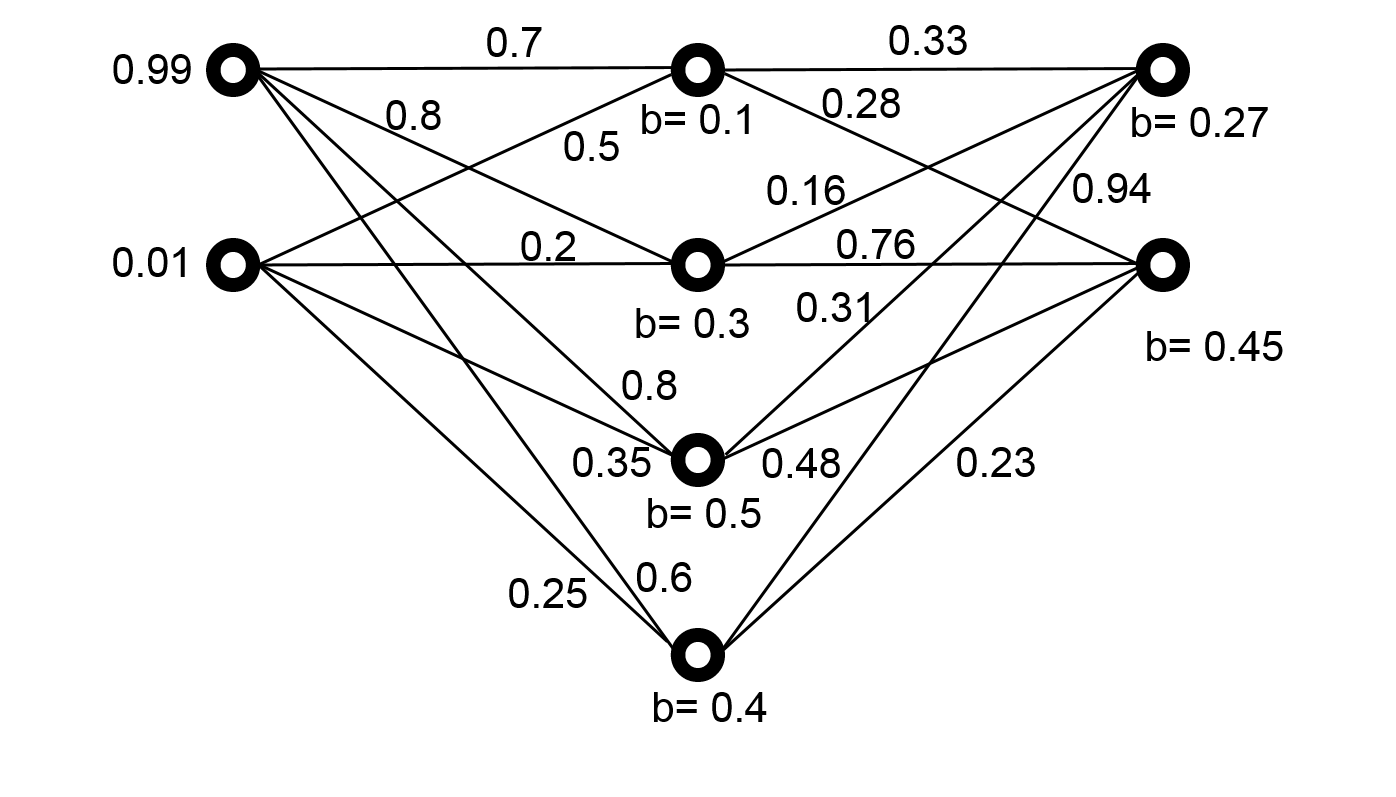
\includegraphics[width=6in]{\thischapterpath/figures/example2.png}}
\caption{A complete example.}
  \label{fig:example2}
\end{figure}

\clearpage
The following program implements this neural network.

\resetlinenumber[1]
\linenumbers
\begin{tt}
  \lstinputlisting{\progpath/supervised/networks/C/example2.c}
\end{tt}
\nolinenumbers

Please validate whether this program correctly implement
Figure~\ref{fig:example2} and produces ouput

\begin{verbatim}
outputs[0] = 0.824528, outputs[1] = 0.852863
\end{verbatim}

\section{Logic Gates}


\begin{figure}[h]
\centering
{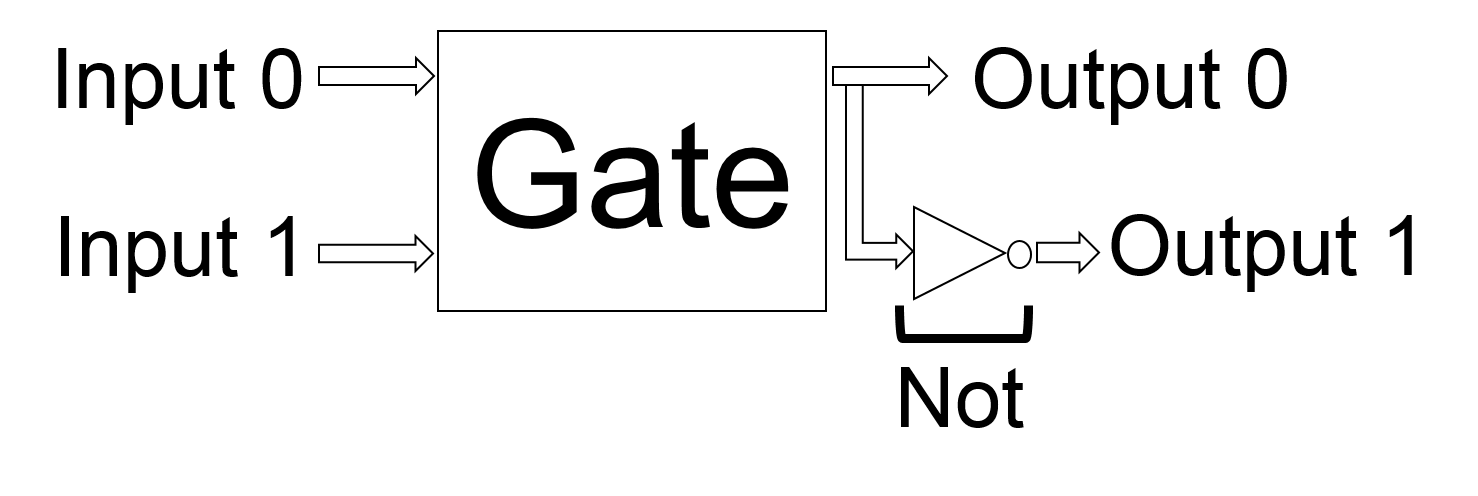
\includegraphics[width=4in]{\thischapterpath/figures/gate.png}}
\caption{A logic gate with two inputs and two outputs.}
  \label{fig:gate}
\end{figure}

Figure~\ref{fig:gate} shows the logic gate to be created in this
assignment.  The logic gate has two independent inputs (called input0
and input1).  One of the outputs is a typical logic gate (AND, OR,
XOR) and the other output is the negation of the first output (after
passing a NOT gate).  Table~\ref{table:logicgates} shows the expected
outputs of the three types of gates.

\begin{table}
\begin{tabular}{|c|c||c|c||c|c||c|c||}  \hline
\multirow{2}{*}{\bf Input 0} &
\multirow{2}{*}{\bf Input 1} &
\multicolumn{2}{c||}{\bf AND} &
\multicolumn{2}{c||}{\bf OR} &
\multicolumn{2}{c||}{\bf XOR} \\
& & {\bf Output 0} & {\bf Output 1} &
{\bf Output 0} & {\bf Output 1} &
{\bf Output 0} & {\bf Output 1} \\ \hline

false & false & false & true & false & true & false & true \\ \hline

false & true & false & true & true & false & true & false \\ \hline

true & false & false & true & true & false & true & false \\ \hline

true & true & true & false & true & false & false & true \\ \hline
\end{tabular}
\caption{Logic gates and the expected outputs.}
\label{table:logicgates}
\end{table}

The output of the sigmoid function is between 0 and 1.  Thresholds can
be set to interpret the values as true or false.  For example, any
value less than 0.2 is interpreted as false; any value greater than
0.8 is interpreted as true.  Based on the thresholds, both outputs of
the example in Figure~\ref{fig:example2} are true and this is
incorrect for any of the three gates.  To produce correct outputs, the
weights must be adjusted.  This assignment does not discuss how to
adjust biases.

\section{Back Propagation Between Hidden and Output Layers}

This assignment uses {\it training} to adjust the weights.
Figure~\ref{fig:example2}'s outputs are different from the expected
values.  This is an example of {\it supervised learning}.  Supervised
learning means that for the given inputs, the correct outputs are
known.

When the outputs are different from the expected results, the
difference is called the {\it error}.  Let's use $\mathds{E}$ to
express the error and $\mathscr {\bf e}_{l, d}$ be the expected ouput
of neuron $d$ at layer $l$ ($l$ is 2 for the outputs in
Figure~\ref{fig:example2}).  Many different ways have been proposed
for defining the error. The sum of square differences is the most
commonly used:

\begin{equation}
\mathds{E} =
\frac{1}{2} \underset{d}{ \Sigma} (\mathscr {\bf e}_{l, d}
- \mathscr {\bf o}_{l, d})^2.
\label{eqn:error}
\end{equation}

The constant $\frac{1}{2}$ is here for convenience because it will be
cancelled later.  In Figure~\ref{fig:example2}, if the desired gate is
AND, the error is

\begin{equation}
\frac{1}{2} ((0 -  0.824528) ^ 2 + (1 - 0.852863)^2)) = 0.350748.
\end{equation}

This calculation uses 0 and 1, instead 0.2 and 0.8, so that the error
is larger and can accelerate learning.

This assignment uses {\it gradient descent} to correct the errors.
This concept is from Calculus (please review Calculus if necessary).
The relationship between $\mathds{E}$ and a particular weight $w$ can
be expressed as a function.  Since the value of $w$ can change by
small amounts (it is double-precision floating point), this function
can be thought of as continuous.  The speed of change in $\mathds{E}$
at this weight $w$ is defined as the {\it gradient}:

\begin{equation}
\nabla \mathds{E} = \frac{\partial \mathds{E}}{\partial w}.
\end{equation}

When $w$ changes by a small amount $\Delta w$,
$\mathds{E}$ is changed by

\begin{equation}
\Delta \mathds{E} = \nabla \mathds{E} \cdot \Delta w.
\label{eqn:deltaE}
\end{equation}

Learning means the error becomes smaller. Thus, it is desirable to
find $\Delta w$ such that $\Delta \mathds{E}$ is negative.
One way to do that is by setting

\begin{equation}
\Delta w = - \eta \nabla \mathds{E}.
\end{equation}

Replacing $\Delta w$ in (\ref{eqn:deltaE}):

\begin{equation}
\Delta \mathds{E} = - \eta (\nabla \mathds{E})^2.
\end{equation}

This ensures that $\Delta \mathds{E}$ is negative and $\mathds{E}$
becomes smaller.  The value $\eta$ is called the {\it learning rate}.
Its value is usually between 0.1 and 0.5.  If $\eta$ is too small,
$\Delta \mathds{E}$ changes very slowly, i.e., learning is slow.  If
$\eta$ is too large, (\ref{eqn:deltaE}) may no longer be correct.

When people study machine learning, they often get confused about how
to calculate the derivative of $\mathds{E}$ with respect to a weight
$w$.  $\mathds{E}$ is not explicitly defined as a function of
$w$---like the examples in most Calculus textbooks.  {\it This does
not matter} because it is not necessary to express $\mathds{E}$ as a
mathematical function of $w$.  As (\ref{eqn:derivativesigma}) shows,
when the $\sigma$ function is used, the derivative depends on only the
value of the output.  Thus, if you know  $\mathds{E}$,
you also know $\nabla \mathds{E}$.

Now, the question becomes how to calculate $\nabla \mathds{E}
= \frac{\partial \mathds{E}}{\partial w}$.  The goal is to determine
what value a particular weight $w_{l-1, s, d}$ needs to be changed by
finding the partial derivative of $\mathds{E}$ with respect to this
weight.  To compute $\nabla \mathds{E}$ for this weight, the {\it
chain rule} is used.  Suppose $y = f(u)$ is a differentiable function
of $u$ and $u = g(x)$ is a differentiable function of $x$. Then,

\begin{equation}
\frac{dy}{dx} = \frac{dy}{du} \cdot \frac{du}{dx}.
\end{equation}

It can be written in a different way:

\begin{equation}
(f \circ g)'(x) = f'(g(x)) \cdot g'(x).
\end{equation}

What does this mean?  The derivative of a composite function can be
obtained by taking derivatives one at a time.

Equation (\ref{eqn:error}) defines the error in terms of the outputs
and the expected values.  The expected values are given by the
learning examples and they are constants.  The weight $w_{l-1, s, d}$
affects only the output of neuron $d$, $\mathscr {\bf o}_{l, d}$.
Consequently, the error needs to consider only $\mathds{E}
= \frac{1}{2} (\mathscr {\bf e}_{l, d} - \mathscr {\bf o}_{l,
d})^2$. Please notice that $\Sigma$ has been removed.

\begin{equation}
\frac{\partial \mathds{E}}{\partial w_{l-1, s, d}}
= \frac{\partial \mathds{E}} {\partial \mathscr{\bf o}_{l, d}} \frac{\partial
\mathscr{\bf o}_{l, d}}{\partial w_{l-1, s, d}}.
\label{eqn:partialEoutput}
\end{equation}

\begin{equation}
\frac{\partial \mathds{E}} {\partial \mathscr{\bf o}_{l, d}}
= (\mathscr{\bf o}_{l, d} -   \mathscr{\bf e} _{l, d}).
\end{equation}

Let
\begin{equation}
x = b_{l, d} + \underset{t}{\Sigma} (w_{l-1, t, d}
\cdot \mathscr{\bf o}_{l- 1, t}).
\label{eqn:definex}
\end{equation}

Then,
$\mathscr{\bf o}_{l, d} = \sigma(x)$.
The derivative is

\begin{equation}
\frac{\partial
\mathscr{\bf o}_{l, d}}{\partial w_{l-1, s, d}}
= \frac{\partial \mathscr{\bf o}_{l, d}} {\partial x}
 \frac{\partial x} {\partial w_{l-1, s, d}}
= \sigma(x) (1 - \sigma(x)) \frac{\partial x} {\partial w_{l-1, s, d}}.
\end{equation}

Finally, 

\begin{equation}
\frac{\partial x} {\partial w_{l-1, s, d}} =  \mathscr{\bf o}_{l-1, s}
\label{eqn:partialxwl1}
\end{equation}

Putting everything together and this is the result:

\begin{equation}
\frac{\partial \mathds{E}}{\partial w_{l-1, s, d}}
= (\mathscr{\bf o}_{l, d} -   \mathscr{\bf e} _{l, d}) \cdot \mathscr{\bf o}_{l, d} \cdot (1 -
\mathscr{\bf o}_{l, d} ) \cdot  \mathscr{\bf o}_{l-1, s}.
\end{equation}

\begin{equation}
\Delta w_{l-1, s,d} = - \eta (\mathscr{\bf o}_{l, d} -   \mathscr{\bf e} _{l, d}) \cdot \mathscr{\bf o}_{l, d} \cdot (1 -
\mathscr{\bf o}_{l, d} ) \cdot  \mathscr{\bf o}_{l-1, s}.
\end{equation}

This training method is called {\it back propagation}--- using the errors from the
output layer to modify the weights between the hidden layer and the
output layer.  

\section{Back Propagation Between Input and Hidden  Layers}

The previous section considers the weights between the hidden and the
output layers.  Can the same method be applied to the weights between
the input and the hidden layers? The answer is yes but some
modifications are needed.   This section finds the
relationship between error $\mathds{E}$ and weight $w_{l-2, k, s}$.
For consistency, $k$ is used for neuron $k$ at layer $l-2$ and $s$ is
used for neuron $s$ at layer $l-1$ (unchanged).  Equation
(\ref{eqn:partialEoutput}) is changed to

\begin{equation}
\frac{\partial \mathds{E}}{\partial w_{l-2,  k, s}}
= \underset{d}{\Sigma} (\frac{\partial \mathds{E}} {\partial \mathscr{\bf o}_{l, d}} \frac{\partial
\mathscr{\bf o}_{l, d}}{\partial w_{l-2,  k, s}})
= \underset{d}{\Sigma} ((\mathscr{\bf o}_{l, d} -   \mathscr{\bf e} _{l, d}) \frac{\partial
\mathscr{\bf o}_{l, d}}{\partial w_{l-2,  k, s}})
\end{equation}

It is necessary keeping $\underset{d}{\Sigma}$ because $w_{l-2, k, s}$
can affect all neurons at layer $l$, even though $w_{l-2, k, s}$
affects only neuron $s$ at layer $l-1$.
The definition of $x$ is the same as equation (\ref{eqn:definex}).

\begin{equation}
\frac{\partial
\mathscr{\bf o}_{l, d}}{\partial w_{l-2,  k, s}} = \frac{\partial \mathscr{\bf o}_{l, d}} {\partial x}
 \frac{\partial x} {\partial w_{l-2, k, s}} = \sigma(x) (1
 - \sigma(x)) \frac{\partial x} {\partial w_{l-2, k, s}}
 = \mathscr{\bf o}_{l, d} (1 - \mathscr{\bf o}_{l, d}) \frac{\partial
 x} {\partial w_{l-2, k, s}}.
\end{equation}

\begin{figure}[h]
\centering
{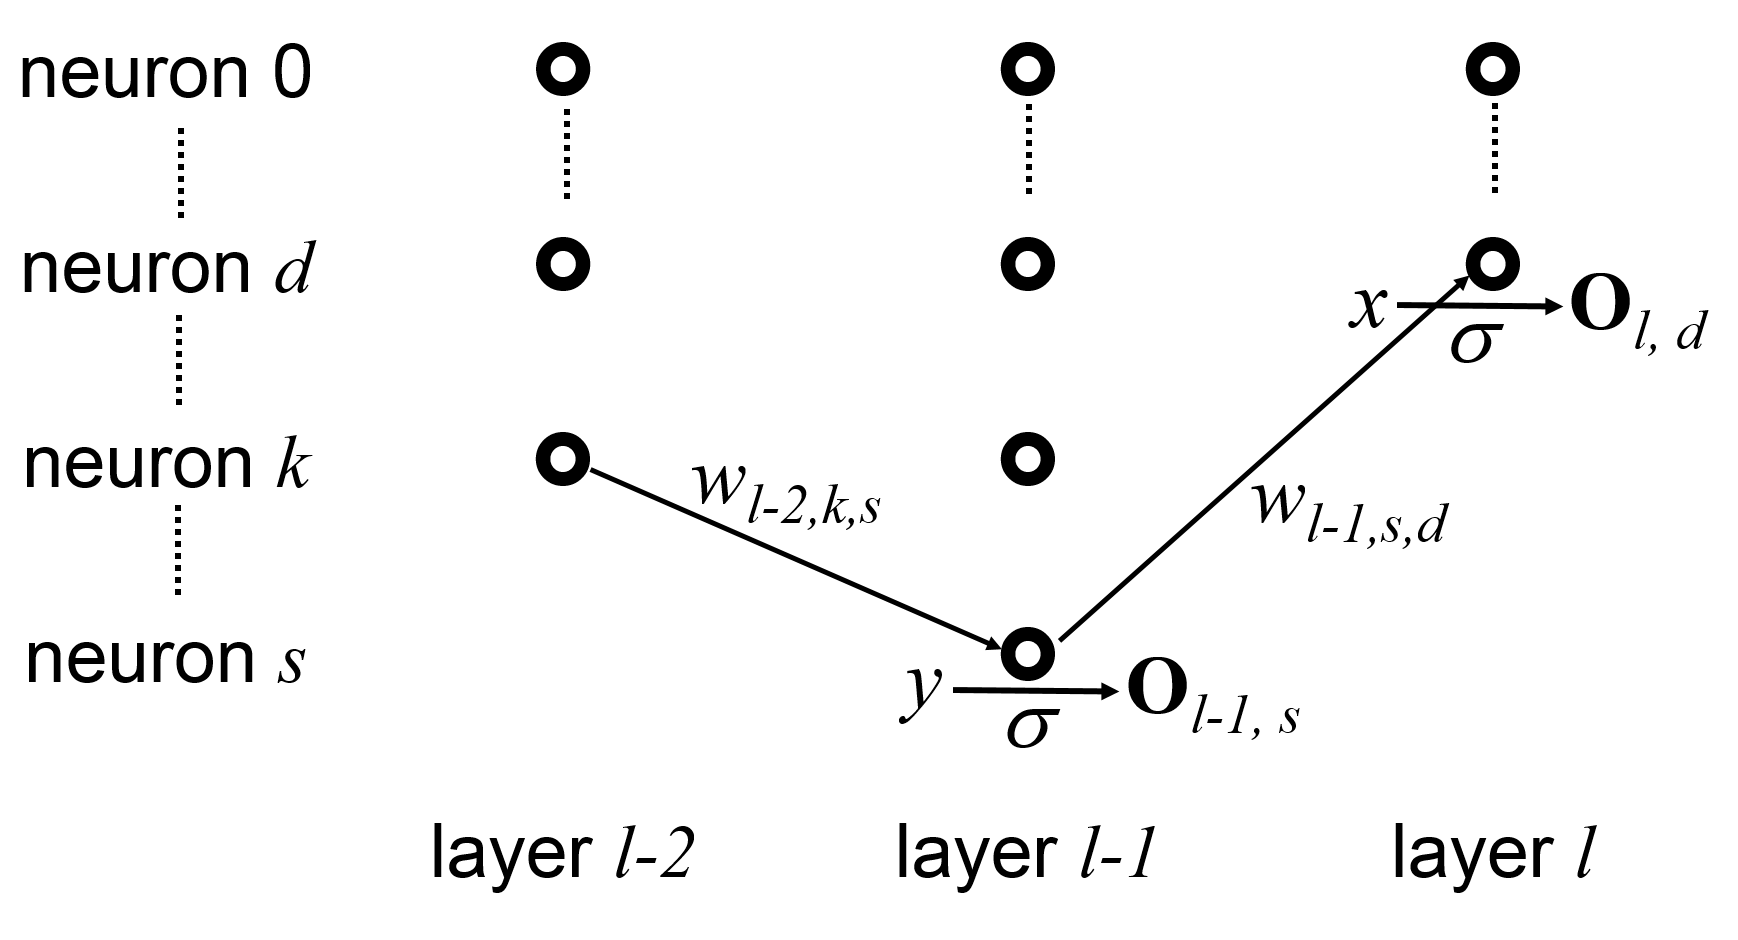
\includegraphics[width=6in]{\thischapterpath/figures/weightl2ks.png}}
\caption{Weight $w_{l-2, k,s}$'s effect.}
  \label{fig:weightl2ks}
\end{figure}


The weight $w_{l-2, k, s}$ affects only the input (and hence the
output) of neuron $s$ at layer $l-1$.


\begin{equation}
\frac{\partial x} {\partial w_{l-2, k, s}} = w_{l-1,  s, d}
\cdot
\frac{\partial \mathscr{\bf o}_{l-1, s}}{\partial w_{l-2,  k, s}}.
\label{eqn:partialxwl2}
\end{equation}

Notice the difference between (\ref{eqn:partialxwl1}) and
(\ref{eqn:partialxwl2}).    Following a similar
procedure by defining

\begin{equation}
y =  b_{l-1, s} + \underset{i}{\Sigma} (w_{l-2, i, s}
\cdot \mathscr{\bf o}_{l- 2,  i}).
\end{equation}

Then,

\begin{equation}
\mathscr{\bf o}_{l-1, t} = \sigma(y)
\end{equation}

and

\begin{equation}
\frac{\partial \mathscr{\bf o}_{l-1, s}}{w_{l-2, k, s}}  =
\sigma (y)(1 - \sigma(y)) \mathscr{\bf o}_{l-2, k}
= \mathscr{\bf o}_{l-1, s} (1 - \mathscr{\bf o}_{l-1, s})
\mathscr{\bf o}_{l-2, k}.
\end{equation}

Putting everything together, this is the relationship between error
$\mathds{E}$ and weight $w_{l-2, k, s}$.

\begin{equation}
\frac{\partial \mathds{E}}{\partial w_{l-2,  k, s}}
= \underset{d}{\Sigma}
(\mathscr{\bf o}_{l, d} -   \mathscr{\bf e} _{l, d})
\mathscr{\bf o}_{l, d}
(1 - \mathscr{\bf o}_{l, d})
 (w_{l-1, s, d} \cdot
 \mathscr{\bf o}_{l-1, s}
  (1 - \mathscr{\bf o}_{l-1, s})
\mathscr{\bf o}_{l-2, k}).
\end{equation}



\begin{equation}
\Delta  w_{l-2,  k, s}
= -\eta \underset{d}{\Sigma}
(\mathscr{\bf o}_{l, d} -   \mathscr{\bf e} _{l, d})
\mathscr{\bf o}_{l, d}
(1 - \mathscr{\bf o}_{l, d})
 (w_{l-1, s, d} \cdot
 \mathscr{\bf o}_{l-1, s}
  (1 - \mathscr{\bf o}_{l-1, s})
\mathscr{\bf o}_{l-2, k}).
\end{equation}

\begin{comment}

\section{Assignment Requirements}

This assignment is different from the other assignments. Instead of
asking you to write a program implementing the equations, this
assignment gives you a program that is already written but contains
some problems (i.e., it has ``bugs'').  You need to submit two files
for this assignment.  The first is a text file explaining how you are
going to find the bugs.  It should provide *details*.  This
explanation needs to clearly describe the plan to identify and fix the
bugs.  The more details, the better. The second file is the corrected
C program.

The explanation should include enough details so that another student
taking ECE 264 is able to repeat what you have done and obtain exactly
the same results.  YOU WILL RECEIVE ZERO IN THIS ASSIGNMENT IF THE
EXPLANATION IS SHORTER THAN 1,000 WORDS.

Your explanation should have enough details so that another student in
the class can recreate your program by reading the explanation,
without reading your code.

Why does this assignment ask you to explain how to debug a program?
Many (perhaps most) students treat debugging as random trial-and-error
without any plan.  This assignment asks you to have a strategy {\it
before} reading the code.

\section{Epilogue}

This assignment gives a simple example as an introduction to
machine learning.  Machine learning is a large field and you can find
dozens of books, thousands of research papers, and hundreds
or online videos, on related topic.

\end{comment}



